\documentclass{beamer}
\usepackage{commath}
\usepackage{hyperref}
\hypersetup{
	colorlinks,
	citecolor=white,
	filecolor=white,
	linkcolor=white,
	urlcolor= cyan
}

\usetheme[progressbar=foot, background=dark]{metropolis}  
\setbeamertemplate{frame footer}{Ankit Pant - 2018201035, Tarun Mohandas 2018201008}

\title{\centering Lipstick on a Pig:
	\\ \vspace{2mm} \normalsize{Debiasing methods cover up systematic gender biases\\ 
		in word embeddings but do not remove them \\ \vspace{3mm} 
		Hila Gonen, Yoav Goldberg} \\ \vspace{-5mm}}
\author{Presented by: \\
	Ankit Pant 2018201035 \\ 
	Tarun Mohandas 2018201008 \\
	Team: \textit{The Lost Linguists}
	}
\date{}
\begin{document}
\begin{frame}[plain]
    \maketitle
\end{frame}
\begin{frame}{Outline}
	\setbeamertemplate{section in toc}[sections numbered]
	\tableofcontents
\end{frame}

\section{Introduction}
	\begin{frame}{Introduction}
		\begin{itemize}
			\item Word Embeddings (WE) - crucial component in for NLP
			\item WEs have been proven to reflect social biases
			\item The paper focuses on Gender Bias
			\item Some work done to reduce gender bias in WE
			\begin{itemize}
				\item Debiasing in post processing step (Bolukbasi et al.)
				\item Debiasing during training (Zhao et al.)
			\end{itemize}
			\item Paper argues that 
			\begin{itemize}
				\item Current debiasing methods mostly hide bias
				\item Lot of bias information can be recovered even after debiasing
			\end{itemize}
		\end{itemize}
	\end{frame}

\section{Gender Bias in Word Embeddings}
	\begin{frame}{Word Embeddings and Gender Bias}
		\begin{itemize}
			\item Word Embeddings
			\begin{itemize}
				\item Most popular representation of document vocabulary
				\item Captures context of words
				\item Various models include \emph{Word2Vec} and \emph{GLoVe}
				\item Both use neural network to form word representations
			\end{itemize}
			\item Gender Bias in Word Embeddings:
			\begin{itemize}
				\item Gender bias of a word $w$ is its projection on the ``gender direction"
				\item $\vec{w}\cdot(\vec{he}-\vec{she})$ (normalised)
				\item Larger projection of $\vec{w}$ on $(\vec{he}-\vec{she}) \implies$ larger bias
			\end{itemize}
		\end{itemize}
		
	\end{frame}

	\begin{frame}{Existing Debiasing Methods}
		\begin{itemize}
			\item Post-processing debiasing (Bolukbasi et al.):
			\begin{itemize}
				\item Make change to word vector to reduce encoded gender bias
				\item Done by zeroing the gender projection of each word on a predefined gender direction
				\item $\vec{w} = \frac{(\vec{w} - \vec{w_b})}{\norm{(\vec{w} - \vec{w_b})}}$
				\item Ensure all neutral words are equally close to the two words
			\end{itemize}
			\item Train word embeddings from scratch (Zhao et al.)
			\begin{itemize}
				\item Alter the loss of GloVe model
				\item Concentrate most gender information to last coordinate of each vector
				\item Use word representation excluding the gender coordinate
				\item Representation of gender neutral words orthogonal to gender direction
			\end{itemize}
		\end{itemize}
	\end{frame}

	
	\begin{frame}{Remaining Bias after using Debiasing methods}
		
		\begin{itemize}
			\item Both methods -- good evidence of removing gender bias
			\item However, they rely on similar specific bias definition:
			\begin{itemize}
				\item ``no gender bias if each non-explicitly gendered word in the vocabulary is in equal distance to both elements of all explicitly
				gendered pairs" (Bolukbasi et al.)
			\end{itemize}
			\item Paper argues that bias is still reflected in similarities between “gender-neutral” words
			\item \textbf{Observation:} ``most word pairs maintain their previous similarity, despite their change in relation to the gender direction."
			\item \textbf{Implication:} Words having specific bias are grouped together
		\end{itemize}
	\end{frame}
	


\section{Experimental Setup}
	\begin{frame}{Experimental Setup}
		\begin{itemize}
			\item Approach consists of two steps:
			\begin{itemize}
				\item For hard-debiasing (Bolukbasi et al.): compare to embeddings before applying debiasing
				\item For GN-GloVe (Zhao et al.): compare to embeddings trained with standard GloVe
			\end{itemize}
			\item Vocabulary:
			\begin{itemize}
				\item Hard-debiased: 26,189 words
				\item GN-GloVe: 47,698 words
			\end{itemize}
			\item Bias is computed for a word by taking its projection on gender direction $\vec{he}-\vec{she}$
,		\end{itemize}
	\end{frame}

	
\section{Experiments and Results}
	\begin{frame}{Clustering of Male and Female Biased words}
		\begin{itemize}
			\item Most biased words in the vocabulary taken
			\item Total 100 words taken (500 male-biased, 500 female-biased)
			\item Clustered into two clusters using \emph{k-means}
			\item For hard-debiasing, alignment accuracy:
			\begin{itemize}
				\item 99.9\% in original biased dataset
				\item 92.5\% in debiased dataset
			\end{itemize}
			\item For GN-GloVe, alignment accuracy:
			\begin{itemize}
				\item 100\% in original biased dataset
				\item 85.6\% in debiased dataset
			\end{itemize}
		\end{itemize}
	\end{frame}
	
	\begin{frame}{Clustering of Male and Female Biased words}
			\vspace{3mm}
			\begin{figure}[htbp]
				\centerline{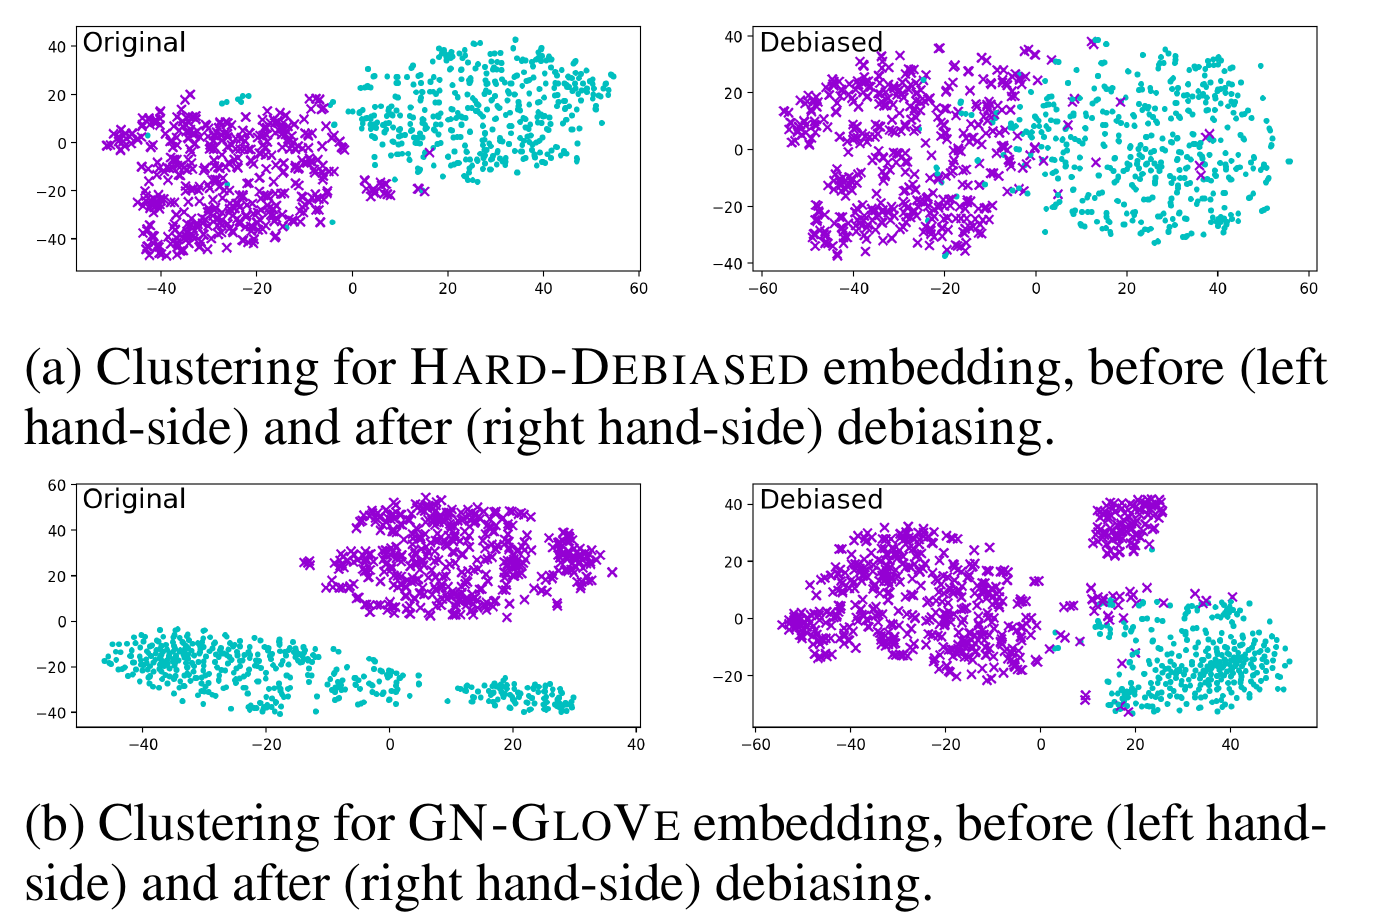
\includegraphics[width=25em]{Cluster_Male_Female_Bias.png}}
				\caption{Result of clustering on male and female biased words}
				\label{bias-cluster-fig}
			\end{figure}
	\end{frame}
	
	\begin{frame}{Bias-by-neighbours}
		\begin{itemize}
			\item Clustering indicates that bias cannot be observed directly
			\item Social bias associated with a word cannot be observed directly in the new embeddings
			\item Can be approximated using the gender-direction in non-debiased embeddings
			\item \textbf{New mechanism}: percentage of male/female socially-biased words among the k-nearest neighbours of the target word
			
		\end{itemize}
	\end{frame}

	\begin{frame}{Professions}
		\begin{itemize}
			\item Considered list of professions used by (Bolukbasi et al.)
		\end{itemize}
		\vspace{3mm}
		\begin{figure}[htbp]
			\centerline{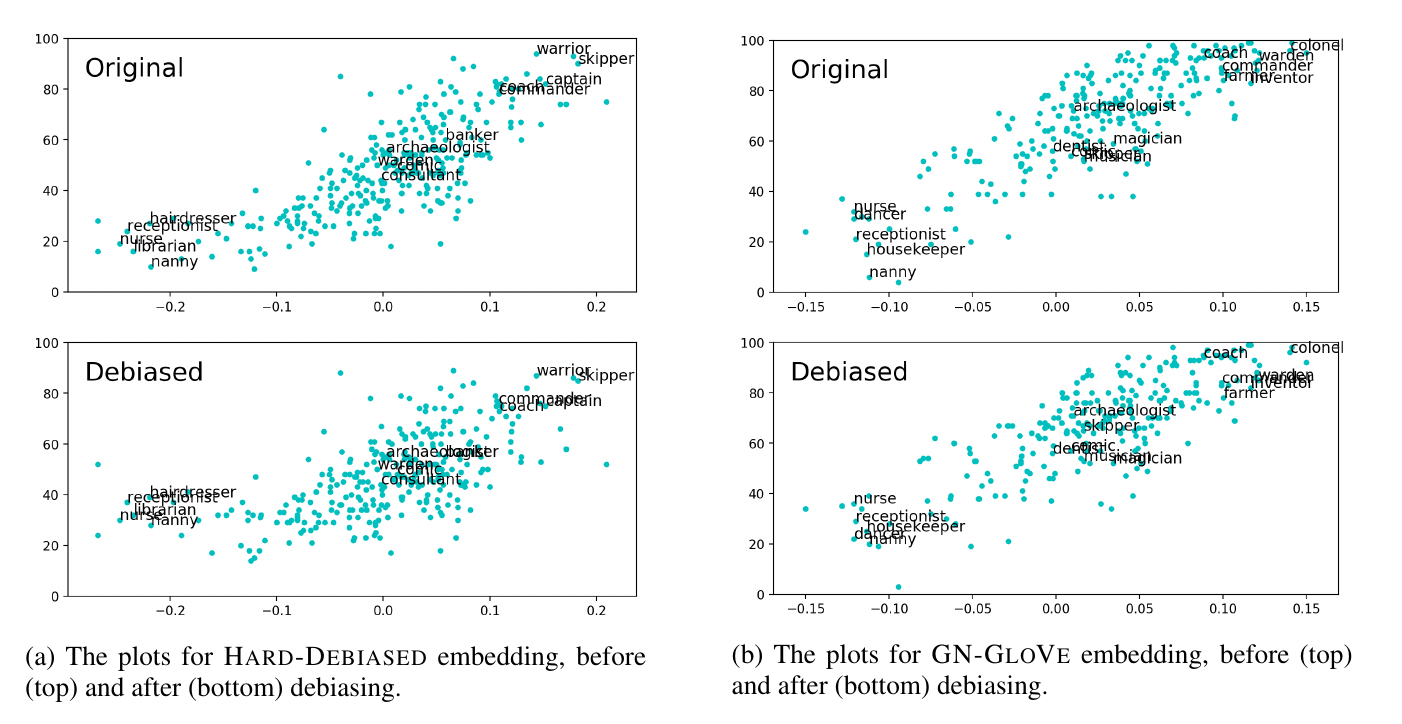
\includegraphics[width=25em]{Cluster_Male_Female_Professions.png}}
			\caption{Result of clustering on male and female professions}
			\label{profession-cluster-fig}
		\end{figure}
	\end{frame}

	\begin{frame}{Classifying biased words}
		\begin{itemize}
			\item Attempt to find if a classifier can be trained to generalise from some gendered words to others
			\item Vocabulary: 5000 words (2500 per gender)
			\item Trained SVM classifier on 1000 random words of vocabulary (500 per gender)
			\item Predict gender for remaining 4000 words
			\item Prediction Accuracy for heard-debiasing:
			\begin{itemize}
				\item 98.25\% for non-debiased data
				\item 88.88\% for debiased data
			\end{itemize}
			\item Prediction Accuracy for GN-GloVe:
			\begin{itemize}
				\item 98.65\% for non-debiased data
				\item 96.53\% for debiased data
			\end{itemize}
			
		\end{itemize}
	\end{frame}


\section{Conclusion}
	\begin{frame}[allowframebreaks]{Conclusion}
		\begin{itemize}
			\item A systematic bias is found in word embeddings even after traditional debiasing
			\item Words with strong bias cluster together
			\item Words having implicit gender will tend to group with other gender-implicit words
			\item Implicit gender of words with prevalent previous gender bias can be predicted from vectors alone
			\item Debiasing methods removes gender direction but it is superficial
			\item  Algorithmic discrimination is more likely to happen by associating one implicitly gendered term with other implicitly gendered terms
			\item Gender-direction measures gender-association of a word but does not determine it
			\item Popular definitions for quantifying and removing bias are not sufficient
		\end{itemize}
	\end{frame}


\section{References}
	\begin{frame}{References}
		\small{
			\begin{thebibliography}{30}
				\bibitem{1} Hila Gonen, Yoav Goldberg, \textit{Lipstick on a Pig: Debiasing methods cover up systematic gender biases in word embeddings but do not remove them}, \url{https://arxiv.org/pdf/1903.03862.pdf}
				\bibitem{2} Tolga Bolukbasi, et al., \textit{Man is to Computer Programmer as Woman is to Homemaker? Debiasing Word Embeddings}, \url{https://arxiv.org/pdf/1607.06520.pdf}
				\bibitem{3} Jieyu Zhao, et al., \textit{Learning Gender-Neutral Word Embeddings}, \url{https://arxiv.org/pdf/1809.01496.pdf}
			\end{thebibliography}
		}
	
	\end{frame}

\end{document}
